% !TeX program = xelatex
% !BiB program = xelatex

\documentclass[landscape,twocolumn,a5paper]{manual}
\usepackage[margin=0.33in,bottom=0.5in,footskip=0.25in]{geometry}

\usepackage{tikz}
\usetikzlibrary{positioning,shapes,backgrounds}
\usepackage{tkz-euclide}
\usepackage{cleveref}

\definecolor{theme}{HTML}{425866}
% \colorlet{theme}{themecolor}

\renewcommand{\arraystretch}{1.5}

\pluginname{ChowKick}
\def\dllink#1{\href{https://chowdsp.com/products.html\#kick}{#1}}

\begin{document}

\section{ChowKick User Manual}

\noindent
\boldtheme{ChowKick} is a kick drum synthesizer based
on creative physical modelling of old drum machine circuits.
The synth contains useful parameters for adjusting the tone
and fundamental frequency of the synthesized kick drum.
The plugin is currently available as a VST/VST3/AU/LV2/AUv3
for Windows, Linux, Mac, and iOS.

\subsection{Installation}
To install ChowKick, download the \dllink{latest release},
and run the installer. If you would like to try the
latest builds (potentially unstable), visit the
\href{https://chowdsp.com/nightly.html\#kick}{Nightly Builds page}.
Note that it is also possible to
\href{https://github.com/Chowdhury-DSP/ChowKick#Building}{compile from the source code}.

\begin{figure}[ht]
    \center
    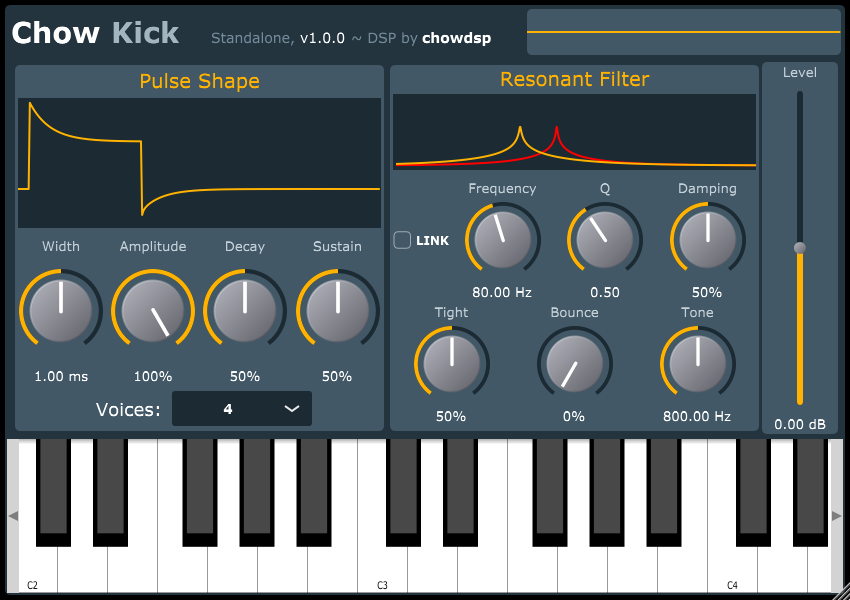
\includegraphics[width=0.75\columnwidth]{screenshots/full_gui.png}
    \caption{\label{fig:full_gui}{\it ChowKick User Interface}}
\end{figure}

\subsection{Controls}
ChowKick contains three main signal processing sections:
a \boldtheme{Pulse Shaper} which generates a synthetic
pulse whenever the kick drum is triggered (see \cref{fig:pulse_shaper}),
a \boldtheme{Noise Generator} which adds noise to the shaped pulse,
and a \boldtheme{Resonant Filter} that creates the kick
drum sound when driven by the pulse.
%
\begin{figure}[ht]
    \center
    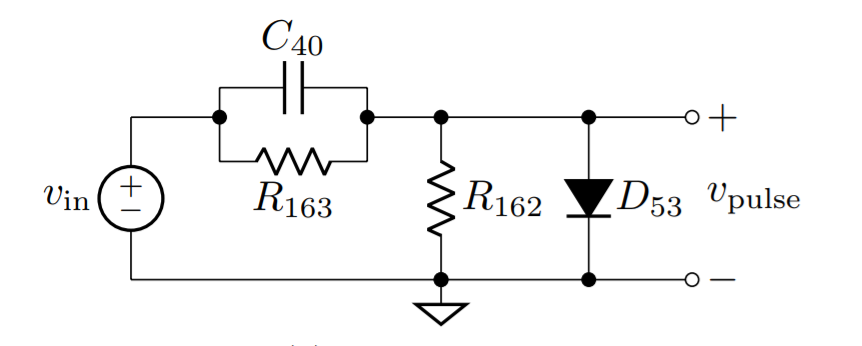
\includegraphics[width=0.65\columnwidth]{figures/pulse_shaper.png}
    \caption{\label{fig:pulse_shaper}{\it TR-808 Pulse Shaper Circuit}}
\end{figure}

\subsubsection{Pulse Shaper}
\boldtheme{Width} controls the width of the generated pulse
used the trigger the kick drum, from 25 microseconds
to 2.5 milliseconds.
\newpar
\boldtheme{Amplitude} controls the maximum amplitude of the
generated pulse used the trigger the kick drum.
\newpar
\boldtheme{Decay} controls how quickly the pulse decays from
its maximum amplitude. Internally, this parameter controls
the value of resistor $R_{162}$ in the pulse shaper circuit.
\newpar
\boldtheme{Sustain} controls the sustain level of the pulse.
Internally, this parameter controls resistor $R_{163}$ in
the pulse shaper circuit.
\newpar
\boldtheme{Voices} controls how many polyphonic voices are
used by the kick synthesizer. This feature can be useful for
kick sounds with a long decay time, so that triggering a new
kick does not cut off the ringing out of the previous kick.
Note that using more voices will not affect the plugin's
CPU usage.

\subsubsection{Noise Generator}
\boldtheme{Noise Amount} controls the amount of noise added to
the shaped pulse.
\newpar
\boldtheme{Noise Decay} controls the decay characteristic of the
generated noise. At 100\%, the noise will decay at the same rate
as the rest of the pulse. At lower valuse, the noise will decay
more quickly than the rest of the pulse.
\newpar
\boldtheme{Noise Cutoff} controls the cutoff frequency of the noise.
\newpar
\boldtheme{Noise Type} controls the type of noise being generated,
including options for \boldtheme{uniform} white noise, \boldtheme{normal}
(or Gaussian) white noise, and \boldtheme{pink} noise.

\subsubsection{Resonant Filter}
The resonant filter section is an implementation of a nonlinear
resonant filter with global feedback.
\newpar
\boldtheme{Frequency} controls the center frequency of the
resonant filter, ranging from 30 Hz to 500 Hz.
\newpar
\boldtheme{Link} disables the frequency control, and instead
uses the plugin's MIDI note input to determine the kick drum's
resonant frequency.
\newpar
\boldtheme{Q} controls the Quality factor of the filter.
\newpar
\boldtheme{Damping} controls the amount of global feedback
around the filter. At low damping values, the kick drum
will have a much longer decay time.
\newpar
\boldtheme{Tight} adjusts the nonlinear characteristic
of the filter so that the filter resonance decreases as
the signal amplitude increases. This parameter can have
a similar effect as using a compressor to ``tighten''
the kick drum sound.
\newpar
\boldtheme{Bounce} adjusts the nonlinear characteristic
of the filter so that the filter frequency increases as
signal amplitude increases. This parameter can be useful
in creating a pitch modulation type of effect for the kick
drum sound.
\newpar
\boldtheme{Tone} adjusts the output tone of the kick drum,
choosing to accentuate or dampen the high frequencies of
the drum sound.
\newpar
\boldtheme{Portamento} adjusts the length of time that
the filter will take to transition from one frequency
to the next.
\newpar
\boldtheme{Res. Mode} controls the way in which the
``tight'' and ``bounce'' affect the overall sound.

\subsection{Tuning}
ChowKick supports full-keyboard microtuning, using the
Scala SCL and KBM microtuning format. The tuning menu
allows you to select .scl and .kbm files to load into
the plugin, as well as an option to reset the plugin
to the standard 12-tone equal temperament tuning (12-TET).
\newpar
For desktop users, you may load tuning files from anywhere
on your computer. A factory library is included with the
plugin, and you may also configure the plugin to use your
own user tuning folder. For iOS users, only the factory
tuning library is available.

\subsection{Presets}
Presets provide a quick way to achieve a specific sound
with the plugin. ChowKick comes with a set of built-in
factory presets. To contribute your presets to be added
to the factory presets list for future releases, please
email me.

\subsubsection{User Presets}
To save the current plugin state as a user preset, open
the presets menu, and select ``Save''. The first time a
preset is saved, you will be asked to choose a preset
folder. All future presets will be saved to this folder,
and when the plugin opens, it will search this folder, as
well as any subfolders, to load new user presets.
Presets located in subfolders will be placed in their
own groups in the preset menu.

\subsection{Open Source}
ChowKick is open-source software that is free (as in ``free
beer''), and free (as in ``free speech''), under the
3-clause BSD license.
\newpar
As an open-source project, ChowKick is
open to outside contributors. If you would like to contribute
to the development of ChowKick, please visit the
\href{https://github.com/Chowdhury-DSP/ChowKick/issues}{issues page}
for a list of outstanding tasks. If you would like to implement
a new feature, please create an issue ticket first, so the
feature can be discussed by the community.

\subsection{Feedback}
If you notice any bugs, or have any questions, feel free
to \href{mailto:chowdsp@gmail.com}{email me directly},
or \href{https://github.com/Chowdhury-DSP/ChowKick/issues}{create an issue ticket}
on GitHub. GitHub issues are preferred, since they are publicly
visible.
\newpar
Enjoy!
\newpar
Jatin Chowdhury
\newpar
\href{https://github.com/Chowdhury-DSP/ChowKick}{https://github.com/Chowdhury-DSP/ChowKick}

\end{document}
